\documentclass[12pt,letterpaper]{article}
\usepackage{graphicx}
\usepackage{ifpdf}

\usepackage{multicol}
\usepackage{tikz}

\usepackage{amssymb}
\usepackage{amsmath}

\usepackage{caption}
\usepackage{subcaption}

\usepackage{hyperref}

\graphicspath{{img/}}

% \usepackage{cite}

%\usepackage[backend=bibtex]{biblatex}
%\bibliography{bibliografia} 

\hypersetup{
    colorlinks=true,
    linkcolor=black,
    citecolor = black,
%     filecolor=magenta,      
    urlcolor=black,
%     pdftitle={GSP Toolbox Manual},
%     bookmarks=true
%     pdfpagemode=FullScreen,
}

\usepackage[spanish]{babel}

\usepackage{fancyhdr}
 
\pagestyle{fancy}
\fancyhf{}
\rhead{Isaac Ayala Lozano\\194520009 \hspace{2 em}   \textbf{\#2}}
\lhead{}
\fancyfoot[R]{\thepage}

\begin{document}
\pagenumbering{gobble}
\section*{Euler-Lagrange}

Se presentan los resultados de la simulación para dos casos de condiciones iniciales: con velocidad angular inicial y sin velocidad angular inicial.
Las condiciones de simulación se muestran en la
tabla \ref{table: initial conditions}. \\

Se observa que la presencia de velocidad angular en el sistema influye considerablemente en el comportamiento general de la esfera al caer.
Para el caso de $\dot \theta$ igual a cero, la esfera cae inmediatamente por el efecto de gravedad (figura \ref{fig:case 3 q lagrange}).
En contraste con este comportamiento, para el caso de $\dot \theta \neq 0$ la esfera nunca cae hacia el fondo del cono.
La posición de la esfera oscila entre los radios de 2 y 3 (figura \ref{fig:case 4 q lagrange}).\\

De los diagramas de fase se identifica que el sistema se encuentra en una órbita alrededor de $r$ sin encontrar un punto de equilibrio (figura \ref{fig:case 3 phase r lagrange}) si la velocidad angular es diferente de cero. 
Para el caso de velocidad angular igual a cero, la posición $r$ decae sin estabilizarse, teniendo un valor máximo en el último instante de simulación.

\begin{table}[h]
\begin{center}
\centering
\begin{tabular}{ccccc}
\hline
Tiempo de simulación & 10 s & & &\\
Masa & 1 kg & $\alpha$ & 1 rad  & \\
\hline
\multicolumn{5}{c}{Condiciones iniciales}\\
 & $r$ & $\theta$ & $\dot r$ & $\dot \theta$\\
Caso 1 & 3 m & 1 rad & 1 $m/s$ & 0 $rad/s$\\
Caso 2 & 3 m & 1 rad & 1 $m/s$ & 1 $rad/s$\\
\hline
\end{tabular}
\end{center}
 \caption{Condiciones de simulación.}
 \label{table: initial conditions}
\end{table}


%%%%%%%%%%%%%%%%%%%%%%%%%%%%%%%%%%%%%%

\begin{figure}
    \centering
    \begin{subfigure}[b]{0.8\textwidth}
        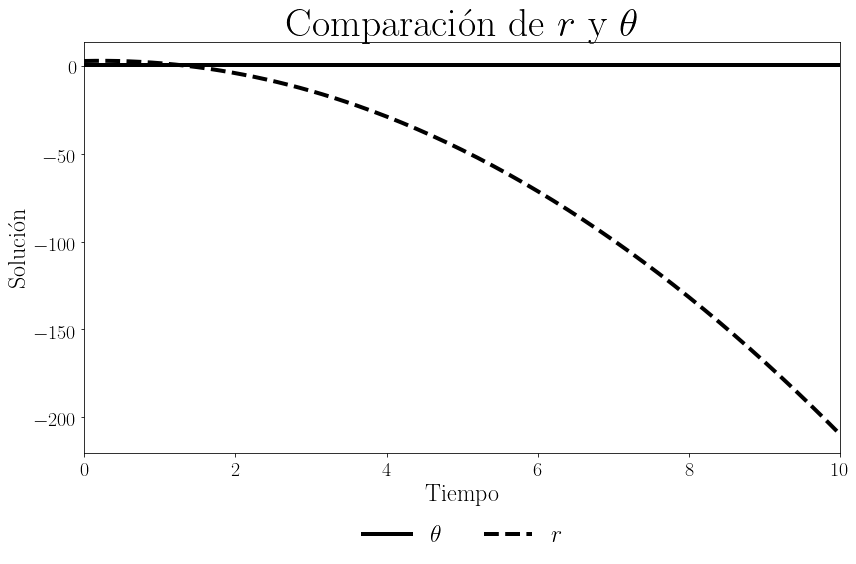
\includegraphics[width=\textwidth]{case03_r_theta}
        \caption{Coordenadas generalizadas $q$.}
        \label{fig:case 3 q lagrange}
    \end{subfigure}
    ~ %add desired spacing between images, e. g. ~, \quad, \qquad, \hfill etc. 
      %(or a blank line to force the subfigure onto a new line)
    \begin{subfigure}[b]{0.8\textwidth}
        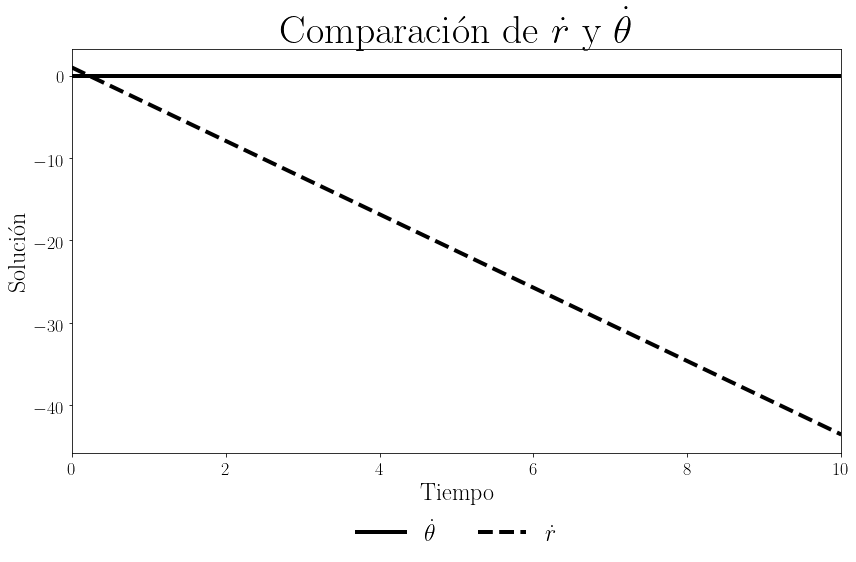
\includegraphics[width=\textwidth]{case03_d_r_d_theta}
        \caption{Primera derivada de coordenadas generalizadas $\dot q$.}
        \label{fig:case 3 dq lagrange}
    \end{subfigure}
    ~ %add desired spacing between images, e. g. ~, \quad, \qquad, \hfill etc. 
    %(or a blank line to force the subfigure onto a new line)
    \caption{Gráfica respecto al tiempo. Caso 1.}\label{fig:case 3 time plot lagrange}
\end{figure}


\begin{figure}
    \centering
    \begin{subfigure}[b]{0.8\textwidth}
        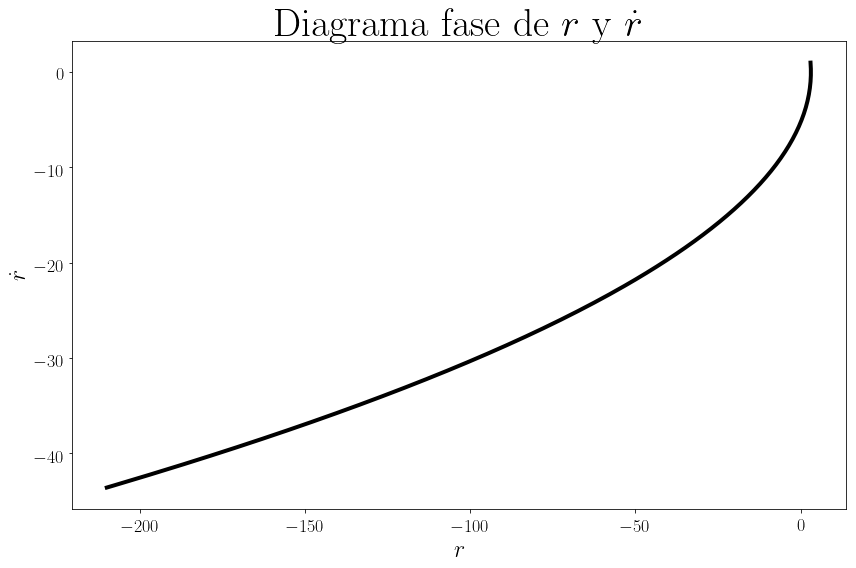
\includegraphics[width=\textwidth]{case03_phase_r_d_r}
        \caption{Posición y velocidad lineal.}
        \label{fig:case 3 phase r lagrange}
    \end{subfigure}
    ~ %add desired spacing between images, e. g. ~, \quad, \qquad, \hfill etc. 
      %(or a blank line to force the subfigure onto a new line)
    \begin{subfigure}[b]{0.8\textwidth}
        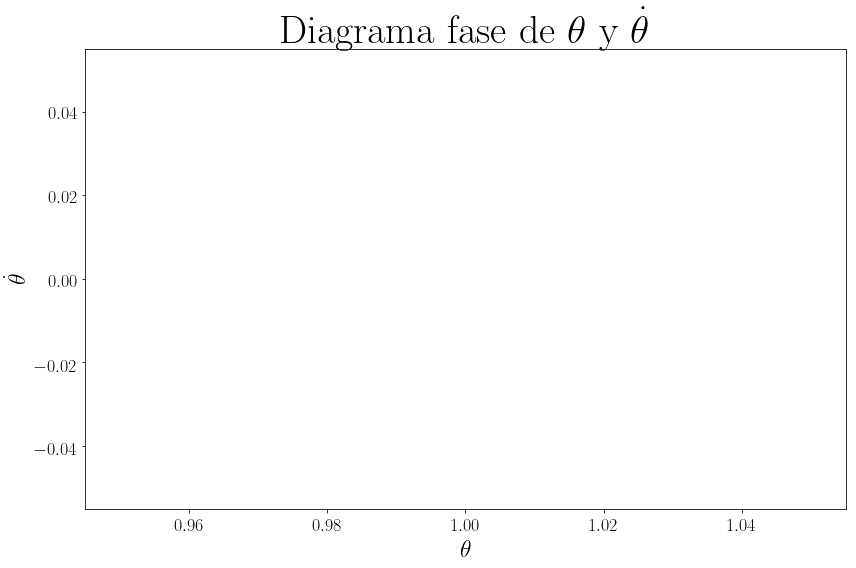
\includegraphics[width=\textwidth]{case03_phase_theta_d_theta}
        \caption{Posición y velocidad angular.}
        \label{fig:case 3 phase theta lagrange}
    \end{subfigure}
    ~ %add desired spacing between images, e. g. ~, \quad, \qquad, \hfill etc. 
    %(or a blank line to force the subfigure onto a new line)
    \caption{Diagramas de fase. Caso 1.}\label{fig:case 3 phase plot lagrange}
\end{figure}

%%%%%%%%%%%%%%%%%%%%%%%%%%%%%%%%%%%%%%

\begin{figure}
    \centering
    \begin{subfigure}[b]{0.8\textwidth}
        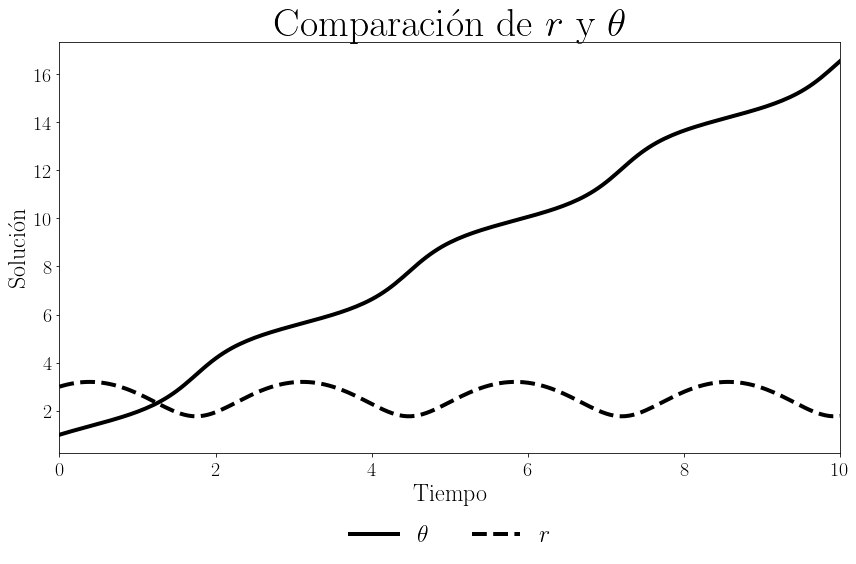
\includegraphics[width=\textwidth]{case04_r_theta}
        \caption{Coordenadas generalizadas $q$.}
        \label{fig:case 4 q lagrange}
    \end{subfigure}
    ~ %add desired spacing between images, e. g. ~, \quad, \qquad, \hfill etc. 
      %(or a blank line to force the subfigure onto a new line)
    \begin{subfigure}[b]{0.8\textwidth}
        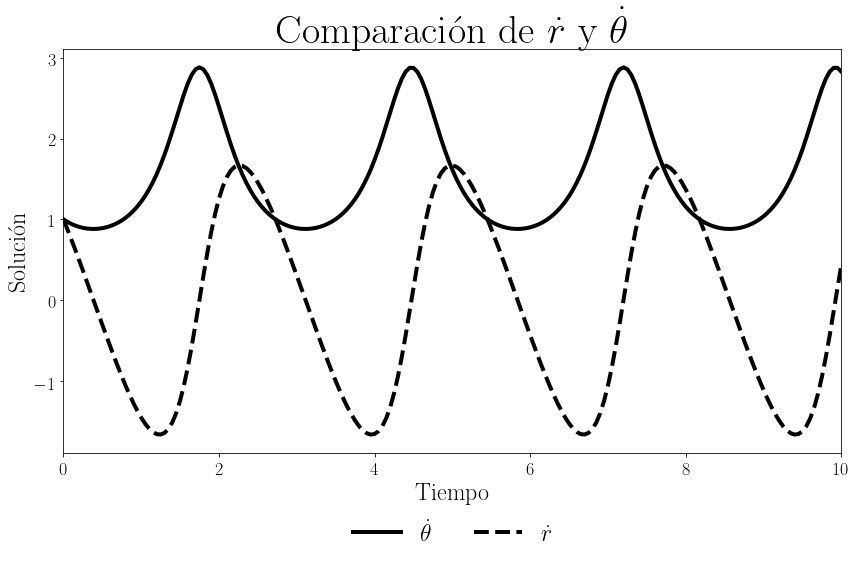
\includegraphics[width=\textwidth]{case04_d_r_d_theta}
        \caption{Primera derivada de coordenadas generalizadas $\dot q$.}
        \label{fig:case 4 dq lagrange}
    \end{subfigure}
    ~ %add desired spacing between images, e. g. ~, \quad, \qquad, \hfill etc. 
    %(or a blank line to force the subfigure onto a new line)
    \caption{Gráfica respecto al tiempo. Caso 2.}\label{fig:case 4 time plot lagrange}
\end{figure}


\begin{figure}
    \centering
    \begin{subfigure}[b]{0.8\textwidth}
        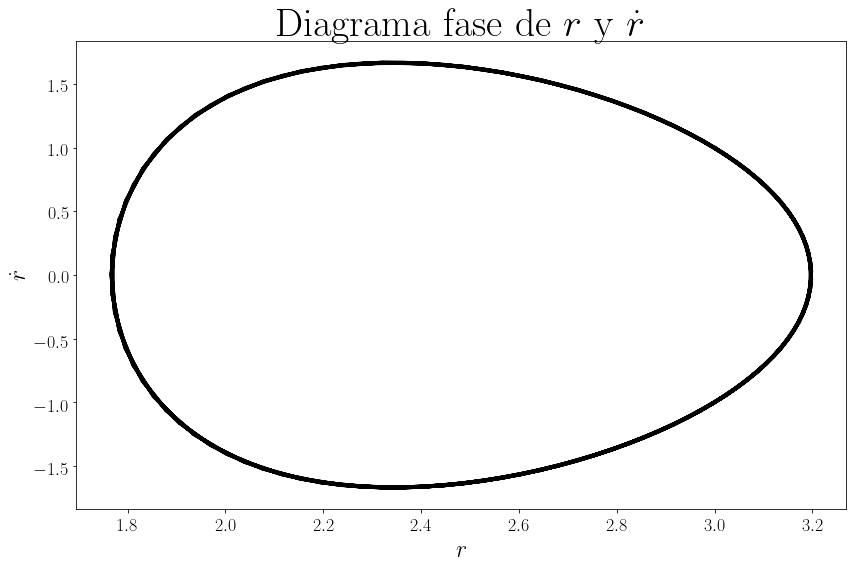
\includegraphics[width=\textwidth]{case04_phase_r_d_r}
        \caption{Posición y velocidad lineal.}
        \label{fig:case 4 phase r lagrange}
    \end{subfigure}
    ~ %add desired spacing between images, e. g. ~, \quad, \qquad, \hfill etc. 
      %(or a blank line to force the subfigure onto a new line)
    \begin{subfigure}[b]{0.8\textwidth}
        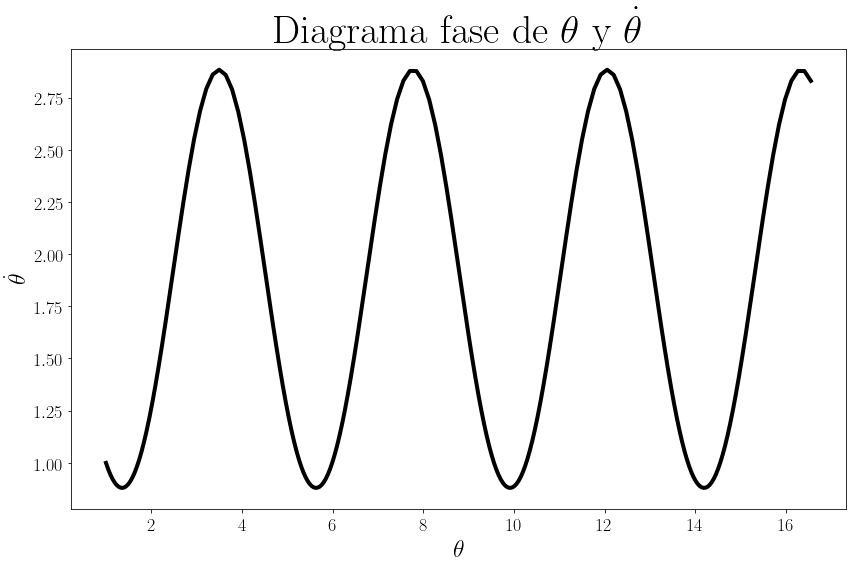
\includegraphics[width=\textwidth]{case04_phase_theta_d_theta}
        \caption{Posición y velocidad angular.}
        \label{fig:case 4 phase theta lagrange}
    \end{subfigure}
    ~ %add desired spacing between images, e. g. ~, \quad, \qquad, \hfill etc. 
    %(or a blank line to force the subfigure onto a new line)
    \caption{Diagramas de fase. Caso 2.}\label{fig:case 4 phase plot lagrange}
\end{figure}

%%%%%%%%%%%%%%%%%%%%%%%%%%%%%%%%%%%%%%
\pagebreak
\section*{Hamiltoniano}

Se presentan los resultados de la simulación para dos casos de condiciones iniciales: con el componente $p_\theta$ de la cantidad de movimiento (momentum) igual y diferente de cero.
Las condiciones de simulación se muestran en la
tabla \ref{table: initial conditions hamilton}.
Las condiciones de simulación son idénticas a los casos de simulación para el método de Euler-Lagrange.\\

De las figuras \ref{fig:case 3 q hamilton} y \ref{fig:case 4 q hamilton} se observa un comportamiento idéntico del sistema para las variables $r$ y $\theta$.
Los diagramas de fase para $r$ exhiben el mismo comportamiento que en la simulación mediante Euler-Lagrange (figuras \ref{fig:case 3 phase r hamilton} y \ref{fig:case 4 phase r hamilton}).


\begin{table}[h]
\begin{center}
\centering
\begin{tabular}{ccccc}
\hline
Tiempo de simulación & 10 s & & &\\
Masa & 1 kg & $\alpha$ & 1 rad  & \\
\hline
\multicolumn{5}{c}{Condiciones iniciales}\\
 & $r$ & $\theta$ & $p_r$ & $p_\theta$\\
Caso 1 & 3 m & 1 rad & 1 $kg \cdot m/s$ & 0 $kg \cdot m/s$\\
Caso 2 & 3 m & 1 rad & 1 $kg \cdot m/s$ & 9 $kg \cdot m/s$\\
\hline
\end{tabular}
\end{center}
 \caption{Condiciones de simulación.}
 \label{table: initial conditions hamilton}
\end{table}


%%%%%%%%%%%%%%%%%%%%%%%%%%%%%%%%%%%%%%

\begin{figure}
    \centering
    \begin{subfigure}[b]{0.8\textwidth}
        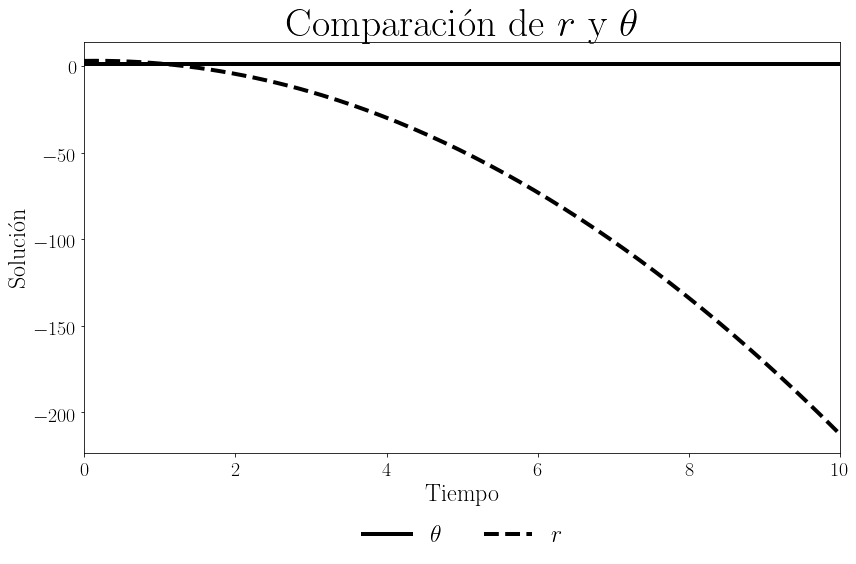
\includegraphics[width=\textwidth]{hamilton_case03_r_theta}
        \caption{Posición linear y angular.}
        \label{fig:case 3 q hamilton}
    \end{subfigure}
    ~ %add desired spacing between images, e. g. ~, \quad, \qquad, \hfill etc. 
      %(or a blank line to force the subfigure onto a new line)
    \begin{subfigure}[b]{0.8\textwidth}
        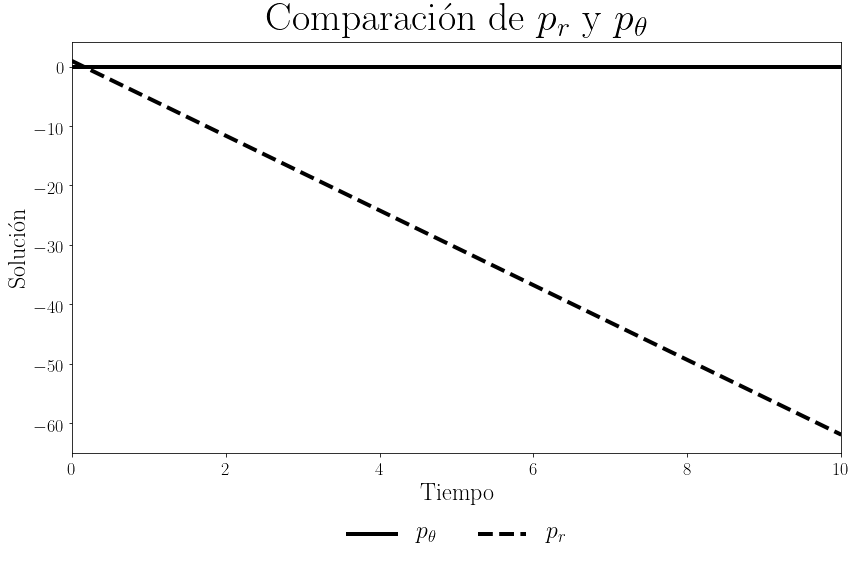
\includegraphics[width=\textwidth]{hamilton_case03_pr_ptheta}
        \caption{Componentes de cantidad de movimiento.}
        \label{fig:case 3 p hamilton}
    \end{subfigure}
    ~ %add desired spacing between images, e. g. ~, \quad, \qquad, \hfill etc. 
    %(or a blank line to force the subfigure onto a new line)
    \caption{Gráfica respecto al tiempo. Caso 1 - Hamiltoniano.}\label{fig:case 3 time plot hamilton}
\end{figure}


\begin{figure}
    \centering
    \begin{subfigure}[b]{0.8\textwidth}
        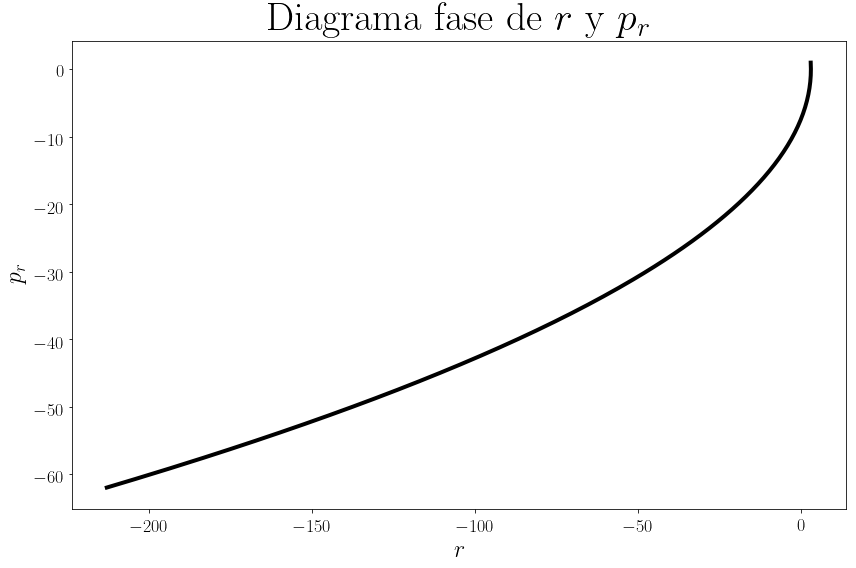
\includegraphics[width=\textwidth]{hamilton_case03_phase_r_pr}
        \caption{Posición linear y componente $p_r$.}
        \label{fig:case 3 phase r hamilton}
    \end{subfigure}
    ~ %add desired spacing between images, e. g. ~, \quad, \qquad, \hfill etc. 
      %(or a blank line to force the subfigure onto a new line)
    \begin{subfigure}[b]{0.8\textwidth}
        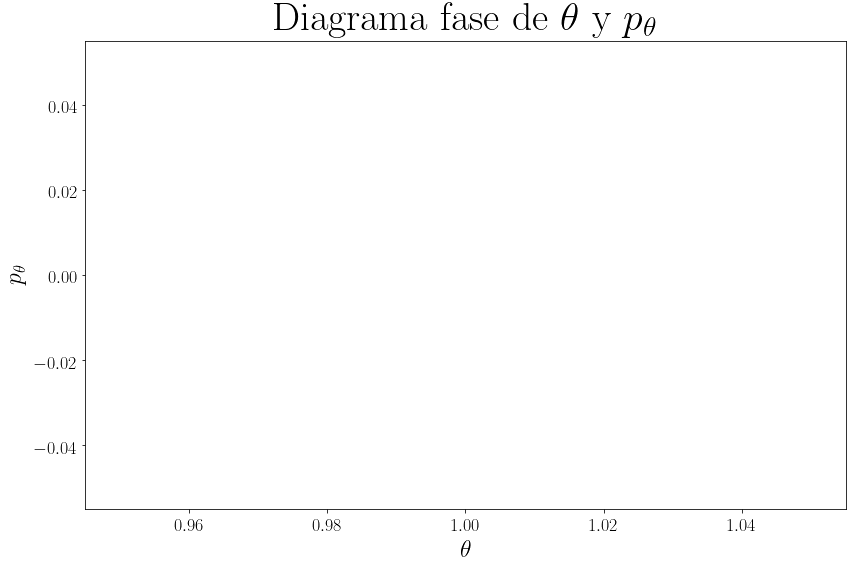
\includegraphics[width=\textwidth]{hamilton_case03_phase_theta_ptheta}
        \caption{Posición angular y componente $p_\theta$.}
        \label{fig:case 3 phase theta hamilton}
    \end{subfigure}
    ~ %add desired spacing between images, e. g. ~, \quad, \qquad, \hfill etc. 
    %(or a blank line to force the subfigure onto a new line)
    \caption{Diagramas de fase. Caso 1 - Hamiltoniano.}\label{fig:case 3 phase plot hamilton}
\end{figure}

%%%%%%%%%%%%%%%%%%%%%%%%%%%%%%%%%%%%%%

\begin{figure}
    \centering
    \begin{subfigure}[b]{0.8\textwidth}
        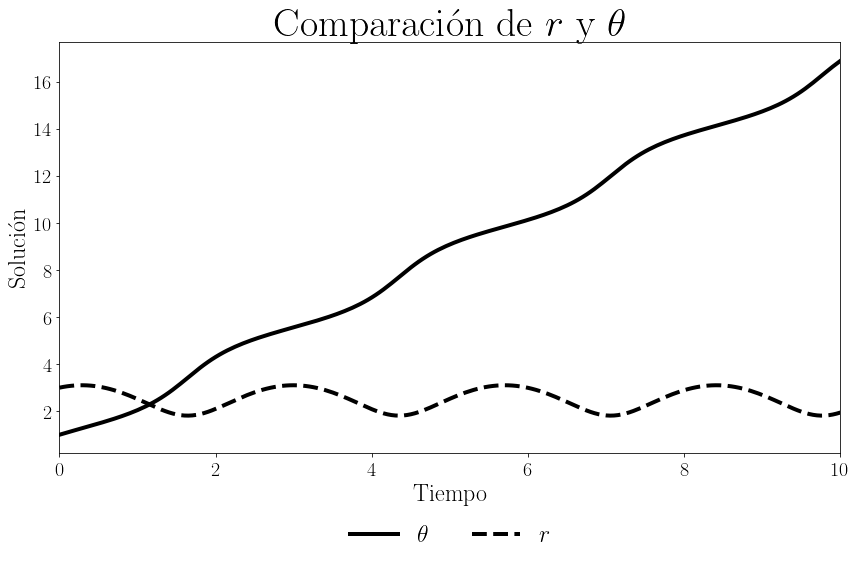
\includegraphics[width=\textwidth]{hamilton_case04_r_theta}
        \caption{Posición linear y angular.}
        \label{fig:case 4 q hamilton}
    \end{subfigure}
    ~ %add desired spacing between images, e. g. ~, \quad, \qquad, \hfill etc. 
      %(or a blank line to force the subfigure onto a new line)
    \begin{subfigure}[b]{0.8\textwidth}
        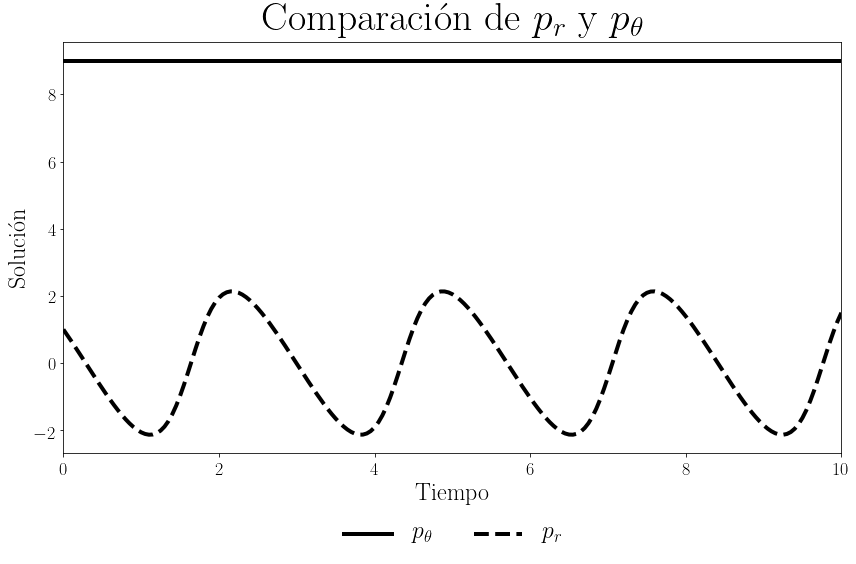
\includegraphics[width=\textwidth]{hamilton_case04_pr_ptheta}
        \caption{Componentes de cantidad de movimiento.}
        \label{fig:case 4 p hamilton}
    \end{subfigure}
    ~ %add desired spacing between images, e. g. ~, \quad, \qquad, \hfill etc. 
    %(or a blank line to force the subfigure onto a new line)
    \caption{Gráfica respecto al tiempo. Caso 2.}\label{fig:case 4 time plot hamilton}
\end{figure}


\begin{figure}
    \centering
    \begin{subfigure}[b]{0.8\textwidth}
        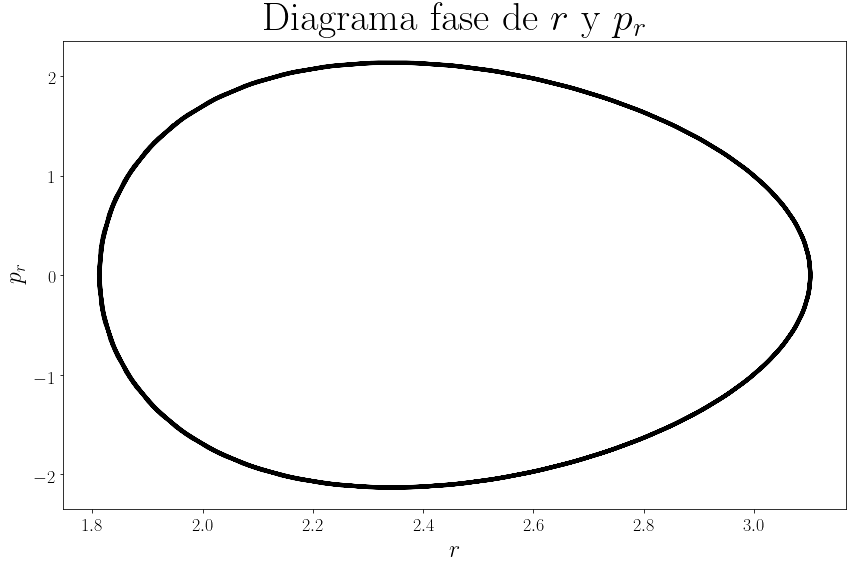
\includegraphics[width=\textwidth]{hamilton_case04_phase_r_pr}
        \caption{Posición linear y componente $p_r$.}
        \label{fig:case 4 phase r hamilton}
    \end{subfigure}
    ~ %add desired spacing between images, e. g. ~, \quad, \qquad, \hfill etc. 
      %(or a blank line to force the subfigure onto a new line)
    \begin{subfigure}[b]{0.8\textwidth}
        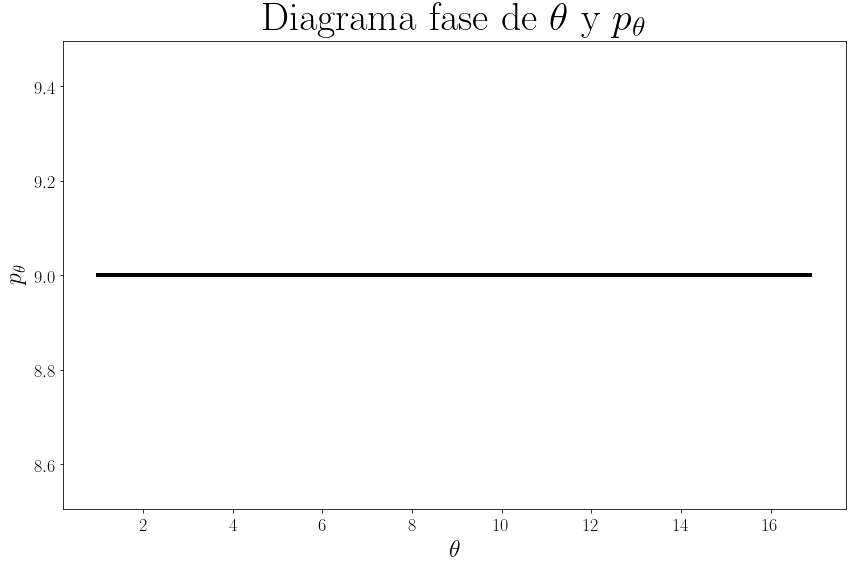
\includegraphics[width=\textwidth]{hamilton_case04_phase_theta_ptheta}
        \caption{Posición angular y componente $p_\theta$.}
        \label{fig:case 4 phase theta hamilton}
    \end{subfigure}
    ~ %add desired spacing between images, e. g. ~, \quad, \qquad, \hfill etc. 
    %(or a blank line to force the subfigure onto a new line)
    \caption{Diagramas de fase. Caso 2 - Hamiltoniano.}\label{fig:case 4 phase plot hamilton}
\end{figure}

%%%%%%%%%%%%%%%%%%%%%%%%%%%%%%%%%%%%%%

\end{document}
